\documentclass[
  letterpaper,
  twocolumn,
  9pt,
  journal,
  final]{IEEEtran}

\usepackage[spanish,es-tabla]{babel}
\usepackage[utf8]{inputenc}
\usepackage{amsfonts}
\usepackage{amsmath}
\usepackage{amssymb}
\usepackage{amsxtra}
\usepackage{mathrsfs}
\usepackage{array}
\usepackage{cite}
\usepackage{varioref}
\usepackage{float}
\usepackage{color}
\usepackage{colortbl}
\usepackage{enumerate}
\usepackage{rotating}
\usepackage{caption}
\usepackage{subcaption}
\usepackage{hyperref}
\usepackage{listings}
\usepackage{lipsum}
\usepackage{flushend}


\title{Tarea 2 - Procesamiento Digital de Imágenes}
% \author{\textbf{Autor:} Pablo Yáñez Santibáñez - pablo.yanez@uai.com}
\author{
  \IEEEauthorblockN{Pablo Yáñez S.} \\
  e-mail: pablo.yanez@uai.cl
}

% Levels to show in table of contents:
% \setcounter{tocdepth}{-1} % only parts
% \setcounter{tocdepth}{0}  % only parts and chapters
\setcounter{tocdepth}{1}  % part,chapters,sections
% \setcounter{tocdepth}{2}  % part,chapters,sections, subsections
% \setcounter{tocdepth}{3}  % part,chapters,sections, subsections,subsubsections
% \setcounter{tocdepth}{4}  % part,chapters,sections, subsections,subsubsections and paragraphs
% \setcounter{tocdepth}{5}  % part,chapters,sections, subsections, subsubsections, paragraphs and subparagraphs.


\begin{document}


\maketitle

\begin{abstract}
We propose \lipsum[1]
\end{abstract}

\tableofcontents

% \listoffigures

% \listoftables


\section{Seccion 1}
\lipsum[1]

\begin{figure}[tbh!]
  \begin{center}
    \resizebox{0.8\columnwidth}{!}{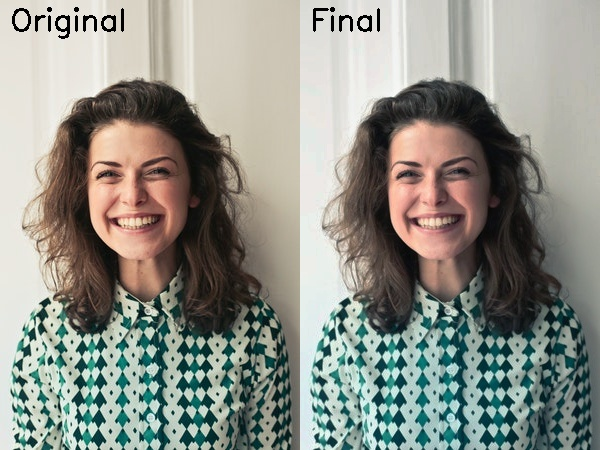
\includegraphics{test_image.jpg}}
  \end{center}
  \caption{Caption 1.} \label{fig:texto referenecia}
\end{figure}

\subsection{Seccion 1.1}
\lipsum[1]

\subsubsection{Seccion 1.1.1}
\lipsum[1]

\section{Seccion 2}

\begin{figure}[tbh!]
  \begin{center}
    \resizebox{0.8\columnwidth}{!}{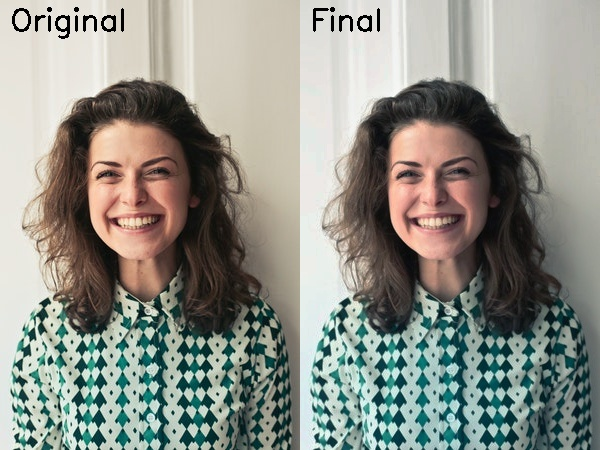
\includegraphics{test_image.jpg}}
  \end{center}
  \caption{Caption 2.} \label{fig:texto referenecia2}
\end{figure}

\lipsum[1]

\begin{table} \caption{A Simple Example Table} \label{table_example}
  \begin{center}
    \begin{tabular}{c c}
      \hline
      \bfseries First & \bfseries Next\\ \hline\hline
      1.0 & 2.0 \\
      \hline
    \end{tabular}
  \end{center}
\end{table}


\section{Seccion 3}


\lipsum[1]

\section{Seccion 4}
\lipsum[1]

\section{Seccion 5}
\lipsum[1]

\section{Seccion 6}

\begin{lstlisting}[language=bash]
  $ wget http://tex.stackexchange.com
\end{lstlisting}


\lipsum[1]

\section{Seccion 7}
\lipsum[1]


\nocite{*}
\bibliographystyle{IEEEtran}
\bibliography{bibliography}


\end{document}



%\begin{figure}[tbh!]
%\begin{center}
%\psfragscanon
%\psfrag{Impulso}[Bc][Br][1.6]{Impulso.}
%\psfrag{Resp impulse}[Bc][Br][1.6]{Respuesta a impulso de $H(z)$.}
%\psfrag{Amplitud}[Bc][Br][1.6]{Amplitud}
%\psfrag{N}[Bc][Br][1.6]{Número de muestra}
%\resizebox{0.5\columnwidth}{!}{\includegraphics{./mfiles/part1/resp_impulse_IIR_parte02.eps}}
%\end{center}
%\caption{Respuesta a impulso del filtro IIR.}
%\label{fig:resp imp IIR}
%\end{figure}

%\begin{lstlisting}[float=tbh!, caption={Magnitud de la respuesta en frecuencia del filtro IIR},label={cod:mag resp frec %IIR}]
%mag=20*log10(abs(H));
%\end{lstlisting}